% IEEE standard conference template; to be used with:
%   spconf.sty  - LaTeX style file, and
%   IEEEbib.bst - IEEE bibliography style file.
% --------------------------------------------------------------------------

\documentclass[letterpaper]{article}
\usepackage{spconf,amsmath,amssymb,graphicx}
\usepackage{graphicx}
\usepackage{tabularx}
\usepackage[export]{adjustbox}
\usepackage{float}
\usepackage{array}


% Example definitions.
% --------------------
% nice symbols for real and complex numbers
\newcommand{\R}[0]{\mathbb{R}}
\newcommand{\C}[0]{\mathbb{C}}

% bold paragraph titles
\newcommand{\mypar}[1]{{\bf #1.}}

% Title.
% ------
\title{Parallel SAT Solving}
%
% Single address.
% ---------------
\name{Jan Eberhardt, Jakub Lichman}
\address{Department of Computer Science\\ ETH Zurich\\Zurich, Switzerland}

% For example:
% ------------
%\address{School\\
%		 Department\\
%		 Address}
%
% Two addresses (uncomment and modify for two-address case).
% ----------------------------------------------------------
%\twoauthors
%  {A. Author-one, B. Author-two\sthanks{Thanks to XYZ agency for funding.}}
%		 {School A-B\\
%		 Department A-B\\
%		 Address A-B}
%  {C. Author-three, D. Author-four\sthanks{The fourth author performed the work
%		 while at ...}}
%		 {School C-D\\
%		 Department C-D\\
%		 Address C-D}
%

\begin{document}
%\ninept
%
\maketitle
%

\begin{abstract}
The boolean satisfiability problem (or SAT) is an interesting problem with various applications.
In this report we describe how we implemented and parallelized a simple SAT solver.
We compare different parallelization variations and analyze their respective trade offs.
We achieved linear or even super linear speedups until up to 28 CPU cores compared to our sequential implementation.
\end{abstract}

\section{Introduction}\label{sec:intro}

\mypar{Motivation}
The boolean satisfiability problem (SAT) belongs to the most important problems in program analysis, verification and other disciplines of theoretical computer science.
It is used in the background of many applications, especially ones in the field of automated planning and scheduling, model checking (formal verification) and theorem proving.
The last decade brought many improvements to the SAT solving world in the form of advanced heuristics, pre-processing and processing techniques, and data structures that allow efficient implementations of search space pruning.
The past 10 years were also rich in improvements in parallelism.
Current trends in computer hardware design decreased performance per processing unit and pack more units on a single processor.
However, algorithms such as DPLL and CDCL were invented before the wide use of parallelism and therefore designed for sequential execution.
Since the SAT problem is NP-complete, we consider it a good candidate to be parallelized.

In our approach, we are trying to speed up SAT solving by running it on multiple cores with different techniques of search space partitioning.

The remainder of this report is structured as follows:
The next subsection provides related work.
In Section \ref{sec:background} we introduce core SAT concepts.
Section \ref{sec:parallel_dpll} explains how we parallelized DPLL and Section \ref{sec:exp} contains the experimental evaluation.
In Sections \ref{sec:discussion}, \ref{sec:futureWork} and \ref{sec:conclusion} we talk about things that we tried that did not work out, about possible extensions to our work and conclude.

\mypar{Related work}
Tomas Balyo et al. proposed the "HordeSat" solver, which can run on up to 1024 cores and is based on the CDCL algorithm.
Their parallel approach is different from ours, because it is portfolio based but with signs of search space partitioning. \cite{hordesat}

Most of the previous SAT solvers designed for computer clusters or grids use explicit search space partitioning.
Examples of such solvers are GridSAT \cite{gridsat}, PMSAT \cite{pmsat} or ManySat \cite{manysat}.

Jurkowiak et al. proposed a work stealing implementation for dynamic load-balancing. \cite{stealing}
Our work stealing approach is similar to what they proposed.

Berger et al. parallelized DPLL in Haskell. \cite{dpll_haskell}
Our DPLL search space partitioning is similar to what they proposed, but our solver is not limited to one machine and we can run on multiple compute nodes.

\section{Background}\label{sec:background}

\mypar{CNF}
A \textit{boolean variable} is a variable that can hold either \textit{true} or \textit{false} as a value.
A \textit{literal} of a boolean variable $x$ is either the positive variable $x$ or its negation $\overline{x}$.
A \textit{clause} is a disjunction (OR) of literals.
A formula in \textit{conjunctive normal form} (CNF) is a conjunction of such clauses.
Every propositional logic formula can be transformed into an equivalent formula in conjunctive normal form.
For the sake of this report we assume that the formula is already in the CNF format.
However a transformation would be simple and straight forward based on basic propositional logic equivalence rules.

\mypar{SAT Solver}
A SAT solver is a program that is able to decide whether a given formula is satisfiable.
More formally, a given formula $F$ is satisfiable \textit{iff} there \textit{exists} an assignment of literals $\theta$ that makes the formula true.
Such a formula $F$ is then called \textit{satisfiable}.
If there does not exits such an assignment, the formula is \textit{unsatisfiable}.
Furthermore, a SAT solver should be able to provide a valid variable assignment in the \textit{satisfiable} case.

\mypar{History}
The first SAT solving algorithm was develop in 1960 by Martin Davis and Hilary Putnam \cite{dp}.
They used a resolution-based decision procedure.
In 1962 Davis, Putnam, Logemann and Loveland developed an extension of the DP algorithm, the DPLL algorithm.
DPLL is a back-tracking-based search algorithm that still forms the basis for many extensions and implementations of SAT solvers.
\begin{figure}
	\centering
	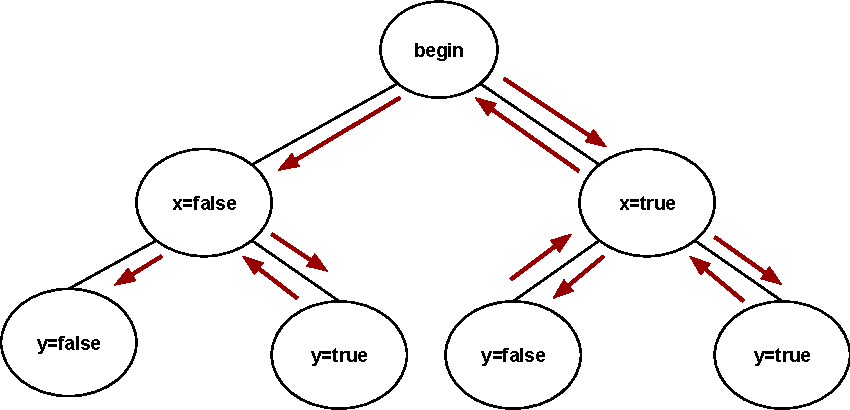
\includegraphics[width=\columnwidth]{figures/dpll_branching.pdf}
	\caption{How DPLL explores the search space of a formula with two variables \textit{x} and \textit{y}.
		\label{fig:dpll-branching}}
\end{figure}

\mypar{DPLL}
DPLL solves a SAT problem by modeling it as a decision tree, variables can either be assigned to \textit{true} or \textit{false}.
In every step DPLL tries to find variables that are "automatically" assigned because of a previous decision,
if there are none it will pick a variable $v_i$ and assume a value for it.
If the path that is taken based on this decision turns out to be unsatisfiable, it backtracks to the decision and picks the negated assignment for variable $v_i$.
The backtracking search continues until a solution is found or the whole decision tree is traversed.
Figure 1 shows how DPLL's decision tree could look like for a simple formula with 2 variables.

\mypar{CDCL}
Similar to DPLL the CDCL algorithm performs a depth-first search on the space of partial truth assignments.
In addition Conflict-Driven Clause Learning (\textit{CDCL}) adopts a pruning technique called learning.
In DPLL it can happen that the same combination of variable assignments results in multiple conflicts and therefore multiple unsatisfiable paths.
CDCL remembers the variable assignments that cause a conflict and avoids them in future decisions, so to say pruning the search space.
This learning is done by analyzing the state whenever a conflict is reached and adding clauses based on that state to the existing formula.
If a conflict cannot be resolved by backtracking, then the formula is unsatisfiable.
If all variables are assigned and no conflict occurred, then the formula is satisfiable.

\section{Parallelizing DPLL}\label{sec:parallel_dpll}

DPLL is a simple backtracking algorithm that explores the search space without any advanced techniques like learning and pruning.
As a result of this, it does not require any transfer of information between stages of solving and therefore it can be nicely parallelized.
The parallelization is not trivial, but far easier than in the case of CDCL, where in addition to load balancing one would need to deal with learned clause sharing.

\mypar{DPLL Branches}
As shown in Figure \ref{fig:dpll-branching} the DPLL algorithm explores the search space with depth first search.
Whenever there are no more variables that can be assigned trivially, one variable assignment is picked.
That is exactly the point where we can do so called DPLL branching: one processor continues on one branch and lets some other processor solve the other branch.
We can call this point a branching point and it represents one node (or decision) in the DPLL decision tree.

The biggest challenge when using this form of branching is load balancing.
The work cannot be split equally between workers at the beginning, because it would require knowledge of the depth of each branch.
This information cannot be inferred from a formula without solving it.
We want to avoid situations where work is not divided equally because we want to fully exploit the computing power of all cores.
In our work we considered two approaches to load balancing.
The first one is a master worker communication model, where one node, called \textit{master}, is in charge of storing partial models and passing them to \textit{workers} that will solve them.
The second approach is a work stealing communication model, where each node (or \textit{worker}) runs on its own and all \textit{workers} are equal.
If some \textit{worker} runs out of work and the formula is not solved yet, it picks a random other \textit{worker} and tries to steal a partial model from it, such that it can continue doing some work.

\mypar{Master Worker Model}
In the master worker model, the \textit{master} is one of the \textit{n} available cores and the other \textit{n-1} cores are \textit{workers}.
At the beginning all workers are marked as free.
The \textit{master} starts solving by passing an empty model to the first free worker.
When a worker reaches a branching point it takes one branch and sends the other\linebreak branch as a partial model to the master.
When the master receives a partial model, it checks whether there exists some free worker.
If not it stores the model into its local stack.
Otherwise it sends it to a worker, which finished solving a branch with \textit{unsat} and therefore is free and needs more work.
This procedure is repeated until some worker finds a \textit{sat} model and sends it to the master.
The master then outputs the model and stops all workers.
If no worker found a \textit{sat} model, the master has an empty stack and all workers are free, then we know that the formula is \textit{unsat}.

While the master worker model is easy to understand and implement, it comes with several drawbacks.
The first of them is the lack of one core.
In the master worker model, one core (the master) is only used as a manager and therefore this core is not actually doing any computation.
The next issue is related to scaling.
The master can become a bottleneck with a certain number of cores, because there is too much communication it needs to process.
As a result workers need to wait longer for getting new partial models.
The last problem is also related to the amount of communication in this model.
Partial models and meta data are transferred every time a worker branches or requests a new partial model.

\mypar{Work Stealing Model}
Because of the drawbacks mentioned above we have decided to reduce and decentralize the communication by implementing a work stealing model.
The model treats all cores \textit{equally} and therefore there is \textit{no master}, just workers.
All workers contain their own stacks with partial models to be processed.
This reduces the communication overhead because all produced models are stored locally instead of sending them to and storing them at the master.
However, the existence of this local stack breaks load balancing because some workers can work on bigger subtrees of the search space than the others.

Inequalities in load balancing are resolved by a mechanism called work stealing.
If some worker finished its work and no other worker has solved the formula yet, than it tries to "steal" a partial model from one of the other workers.
The process of stealing can be defined as follows:
A worker tries to steal from a randomly selected other worker until it finds a model or until someone else has found one.
There are two more phases in the communication model.
The first phase is the initial work distribution and the third one is the stopping criteria.
In the first phase worker 0 will take the role of the master and distribute starting models to all other workers.
Then all workers will try to solve their subtrees and in the case of running out of work they will try to steal work from some other worker (phase 2).
When some worker finds a \textit{sat} model, it will send it to worker 0, who stops all workers and outputs the final model (phase 3).
A master is necessary at the end because there can be multiple workers that find a \textit{sat} model at the same time.
In our implementation, worker 0 prints the first obtained \textit{sat} model and ignores the others.

Our current work stealing implementation has one drawback:
It can only handle satisfiable formulas.
The stopping criteria in the unsatisfiable case was very trivial in the master worker model because there exists a moment when the stack at the master was empty and all workers were free.
In the work stealing model, no such moment exits.
We do not have a central node that controls the others and so knows in which stage each worker is and therefore we restrict ourselves just to satisfiable formulas with this communication model.

\mypar{Implementation}
We implemented both communication models in C++ with the help of MPI \cite{mpi}.
Our DPLL solver is implemented in C++ as well and therefore we can directly interact with MPI from within the solver.
We tried to keep the implementation of the DPLL algorithm and communication within nodes as separate as possible for better readability.
We used \textit{vector}s from the C++ standard library to represent sets of clauses and sets of literals.
We used \textit{unsigned int}s as variable names, and \textit{boolean} types for sign and value of the literals and variables.
To implement the backtracking algorithm we used recursion, but we allocate all necessary data structures on the heap.
We did not experience any stack overflow issues.

\mypar{Correctness}
We tested our sequential DPLL solver on hundreds of formulas that we either randomly generated or took over from a SATLIB formula collection. \cite{cnf_website}
We ran each formula through z3 \cite{z3} and compared the result of z3 with our result.
The following cases have to be considered for each test case:
If both solvers return unsat, we pass the test case.
If one solver returns sat and the other one unsat, we fail the test case.
If both solvers return sat, we still need to check if the model our solver has returned is correct.
To do that we can conjoin the model to the original formula and again run it through z3.

We ran both parallel implementations through the same set of formulas and checked correctness for each of them.
Assuming that our sequential implementation is correct, it is straight forward that our parallel implementation is correct as well:
we essentially solve the same set of sub problems but on different nodes and in a potentially different order.
The difference between the parallel and stealing version is just the load balancing and not in the searched space.
Both parallel versions solve the same partial models but they are distributed over the working nodes in a different way.

\section{Experimental Results}\label{sec:exp}
In this section we are going to present our experimental results for both of our parallel DPLL models.

\mypar{Experimental Setup}
We ran both communication models on the Euler super compute cluster \cite{euler} on up to 48 cores and requested 1 Gigabyte of memory per core.
48 cores was the maximum number of cores accessible to us.
Euler contains 5 different types of nodes but each of them contains at least two 12-core Intel Xeon processors (2.5-3.7 GHz) and between 64 and 512 GB of DDR4 memory clocked at 1866, 2133 or 2666 MHz.

\mypar{Benchmark Formulas}
During our correctness testing and debugging phase of the core algorithm, we realized that random formulas generated by our own random formula generator are not suitable for performance testing.
Even if we picked formulas that contained the same amount of variables, clauses and literals per clause, we observed large variations in run time between them.
This is caused by the completely random structure of formulas generated by our generator.
Therefore we used a set of 14 formulas taken from a SATLIB formula collection as a benchmark set.
The set contains different real world problems modeled as boolean formulas from various domains such as planning problems,
all-interval series encodings, flat graph coloring, inductive inference, etc.
Our benchmark set also contains a few random formulas that were taken from the SATLIB formula collection as well.
Table \ref{tab:benchmark_set} in the Appendix section contains a detailed listing of the used formulas together with their description.
For the coming subsections we reduced the set of benchmark formulas to a representable subset of size 6 for readability reasons.
We included the corresponding figures for the other 8 formulas in the Appendix section.

\mypar{Master Worker}
We compared the run times of the master worker communication pattern with the sequential version of DPLL.
The achieved speedup is shown in Figure \ref{fig:dpll_parallel_speedup}.
It can be inferred from the figure that the achieved speedup factor heavily depends on the formula.
But it is not just the "size" of the problem or time required to solve a formula with the sequential algorithm that influences the speedup factor.
As shown in Table \ref{tab:cnfs_representatives} the formulas where we reached the highest speedup are not necessarily the ones with the longest time to solve sequentially or the largest number of variables (highest upper bound on the depth of the decision tree).
Note that the best speedup in this subset is achieved for the randomly generated formulas (uf50-01 and uuf50-01).

For the random formulas it is easy to explain why the speedup goes down with more than 32 cores.
The decrease is caused by moments in the solving process where the master is no longer able to serve all the workers at the same time.
Therefore some workers have to wait longer to obtain the next partial model.
This problem starts to occur when the number of cores is larger than 30.
The overall average waiting time of all workers, shown in Figure \ref{fig:dpll_parallel_waiting}, shows this problem.
The waiting time is considered to be the time that some worker spends waiting for a new partial model from the master.
The overall waiting time is the sum of all waiting time periods of all workers, averaged over different runs of the same formula.

For some real world problems the speedup is smaller.
The small speedup is caused by the way the decision tree is traversed.
While the sequential implementation deterministically does a depth-first search and therefore gives us some ordering guarantees,
the parallel version sends all subbranches to the master and gives no ordering guarantees.
It might happen that a worker is "close" to a solution but then receives a partial model in a completely different part of the decision tree that might be unsatisfiable all together.
The size of the subtree where we will not find a solution depends on the structure of the formula.
This is also the explanation why we achieved super linear speedup in some other cases:
There we were lucky enough to reach the final solution with less iterations than in the sequential case.

\begin{figure}[h!]
    \centering
    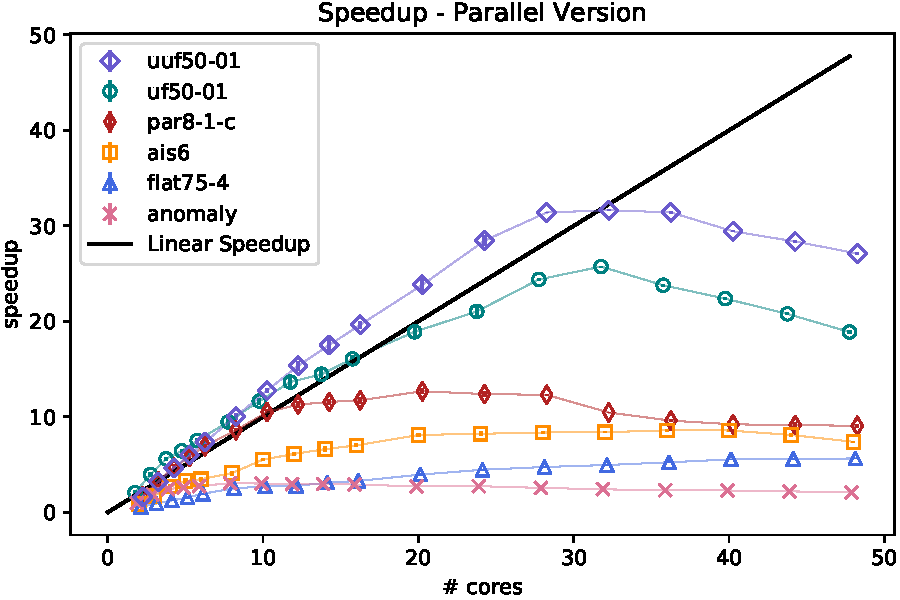
\includegraphics[width=\columnwidth]{figures/scaling_parallel_subset_dpll_scaling_tar.pdf}
    \caption{Average speedup of master worker parallel DPLL implementation compared to sequential DPLL.
    The 95\% confidence intervalls are shown as error bars but too small to be visible in some cases.
    \label{fig:dpll_parallel_speedup}}
\end{figure}
\begin{figure}[h!]
    \centering
    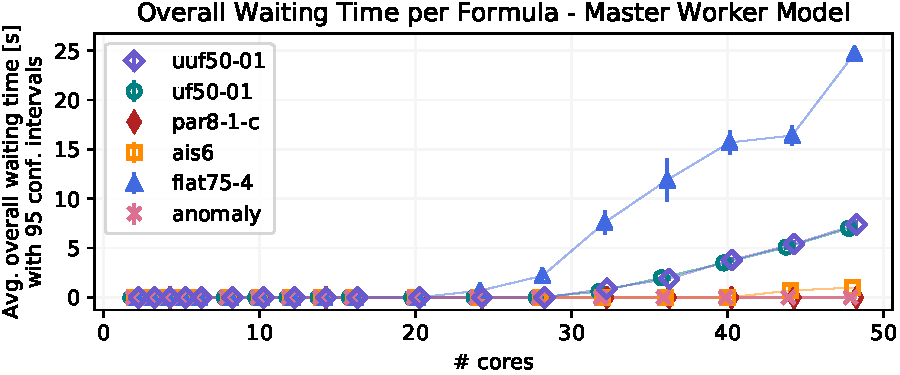
\includegraphics[width=\columnwidth]{figures/waiting_parallel_subset_dpll_scaling_tar.pdf}
    \caption{Average overall waiting time of workers per cnf in the master worker model.
    All waiting times per worker are summed up.
    The 95\% confidence interval are shown as error bars.}
    \label{fig:dpll_parallel_waiting}
\end{figure}
\begin{table}[h!]
    \centering
    \begin{tabularx}{\columnwidth}{|X|c|c|}
        \hline
        Formula & seq. runtime [ms] & \# vars/clauses\\
        \hline
        \hline
        uf50-01 (sat) & 7'890.9 $\pm$ 44.31 & 50/218\\
        \hline
        par8-1-c (sat) & 2'185.0 $\pm$ 32.88 & 64/254\\
        \hline
        ais6 (sat) &  2'964.0 $\pm$ 41.54 & 61/581\\
        \hline
        flat75-4 (sat) & 26'284.6 $\pm$ 172.65 & 225/840\\
        \hline
        anomaly (sat) & 279.7 $\pm$ 6.74 & 48/261\\
        \hline
        uuf50-01 (unsat) & 13'404.2 $\pm$ 102.94 & 50/218\\
        \hline
    \end{tabularx}
    \caption{Overview of sequential runtime of benchmark subset formulas.
    The second column shows the average runtime with the 95 percentiles.}
    \label{tab:cnfs_representatives}
\end{table}

\mypar{Work Stealing}
Similar to the previous comparison, we compared our parallel work stealing model to the sequential DPLL version.
The speedup that we achieved is shown in Figure \ref{fig:dpll_stealing_speedup}.
With the work stealing model we achieved large speedups for a small number of cores but essentially did not gain from adding more cores after some limit.
The reason for this is again the way how we traverse the decision tree.
In theory we should do something that is similar to a global breath first search and local (per node) depth first search in this model.
However because of phase 0 mentioned in Section \ref{sec:parallel_dpll}, the "global breath first" search part is not really a breath first search.
Each worker starts in a node in the decision tree that is one level shifted inwards from the right-most subbranch of the tree.
That means that if the formula is satisfiable, we are guaranteed that at least one worker is working on the correct subtree already after the first decision and will never solve models of the other subtree.

\begin{figure}[p]
    \centering
    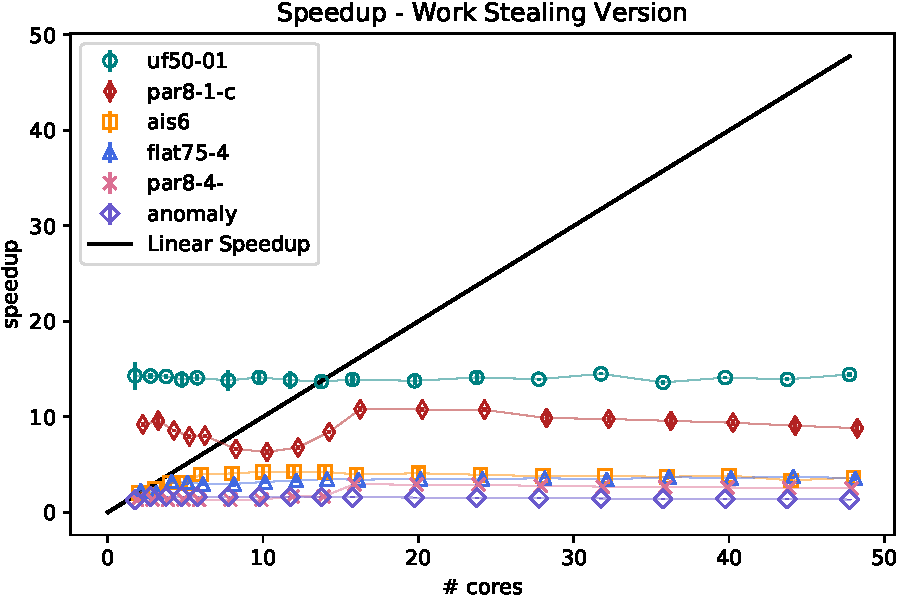
\includegraphics[width=\columnwidth]{figures/scaling_stealing_subset_dpll_scaling_tar.pdf}
    \caption{Speedup of work stealing parallel DPLL implementation compared to sequential DPLL.
    \label{fig:dpll_stealing_speedup}}
\end{figure}
\begin{figure}[p]
	\centering
	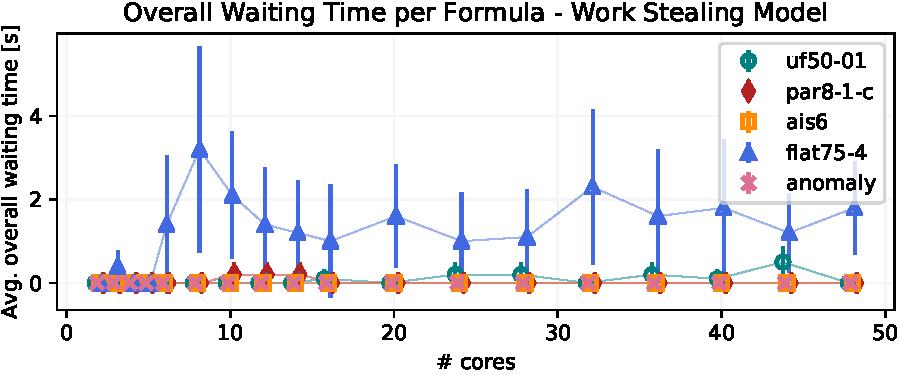
\includegraphics[width=\columnwidth]{figures/waiting_stealing_subset_dpll_scaling_tar.pdf}
	\caption{Average overall waiting time of workers per cnf in the work stealing model.
		All waiting times per worker are summed up.}
	\label{fig:dpll_stealing_waiting}
\end{figure}
\begin{figure}[p]
    \centering
    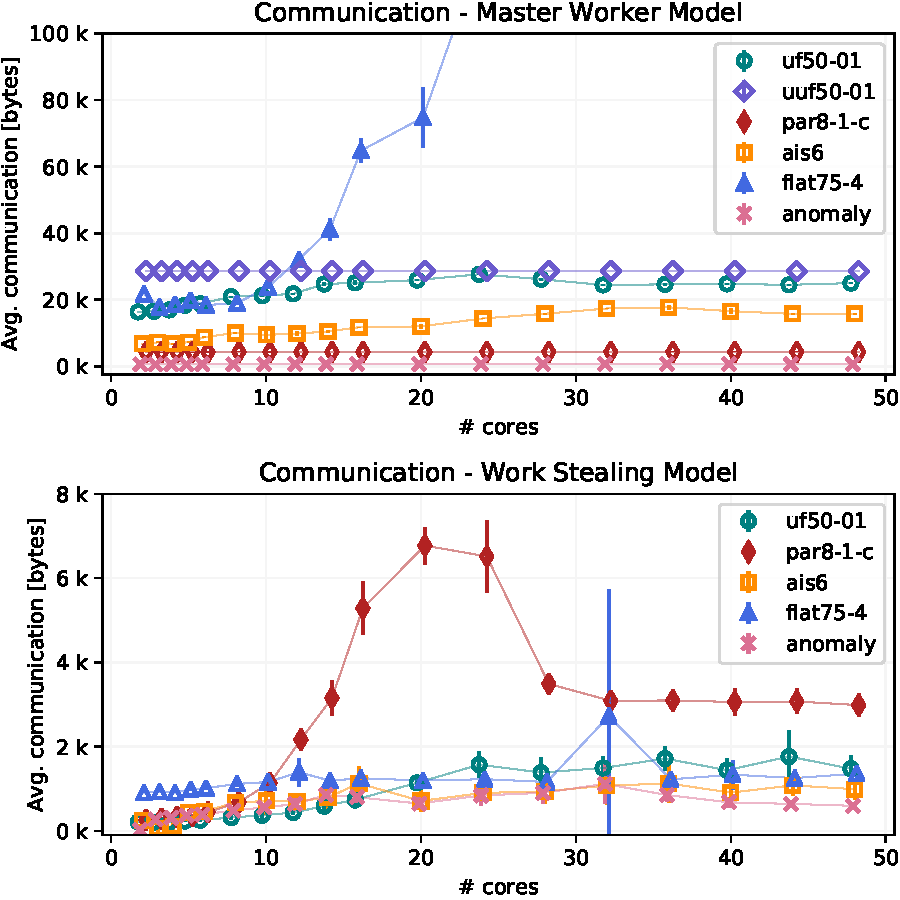
\includegraphics[width=\columnwidth]{figures/comm_subset_dpll_scaling_tar.pdf}
    \caption{Overall amount of transferred bytes for both the master worker model and the stealing model.
    The 95\% confidence intervalls are shown as error bars but too small to be visible for some data points.}
    \label{fig:comm_reduce}
\end{figure}

As an result, we outperform the master worker model with the work stealing model with only a few cores.
But do not gain that much from adding more cores since the search space is split in a non-uniform way.
The overall waiting time of the workers for the work stealing model is shown in Figure \ref{fig:dpll_stealing_waiting}.
The waiting time does no longer go up when increasing the number of cores.

\mypar{Communication Overhead}
One of the reasons why we introduced a work stealing mechanism,
was that it should drastically reduce the amount of communication (bytes transferred) between cores.
Our experimental results prove that and they are shown in Figure \ref{fig:comm_reduce}.
From the upper subplot in Figure \ref{fig:comm_reduce} it can be inferred that the amount of communication is quite high in the master worker model,
but does not necessarily increase when increasing the number of cores.
This constant behavior is caused by the fact that every worker sends every partial model it finds and that it does not directly solve, back to the master,
regardless of the number of cores that are used.
If more cores are used however, it can happen that parts of the decision tree that were not traversed with a smaller number of cores are suddenly traversed.
In the lower subplot of Figure \ref{fig:comm_reduce} the amount of overall communication for the work stealing model is shown.
The amount of communication is reduced, compared to the master worker model.
This reduction is caused by the reduced amount of partial model transfers, as mentioned in Section \ref{sec:parallel_dpll}.
However as we discussed in the previous subsection, the amount of communication is not the only limiting factor.
Master becoming the bottleneck when adding more cores is the main factor.

\section{Discussion}\label{sec:discussion}
In this section we are going to discuss some approaches that we tried during our project but that did not work as expected or we had to stop investigating possible solutions because of time constraints.

\mypar{DPLL-CDCL Hybrid Parallel Solver}
We have implemented a fully working CDCL solver.
Its correctness was proven with the same testing infrastructure that we use to test our DPLL implementation.
The sequential version of the CDCL solver was faster than the sequential DPLL implementation for all of our benchmark formulas.
Quite naturally we tried to plug that solver in locally at the workers to boost the performance.
The way we did it is the following:
First we run DPLL in parallel (it does not matter which of the two communication patterns we pick) and we only branch a certain number of times per worker.
After that "branching limit" is reached we switch to CDCL and solve the whole subtree of the original decision tree locally.
When CDCL terminates, we either found a solution or get a new model (either from the master or another worker) and solve it again with CDCL.
This hybrid approach showed worse performance than we expected.
The reason for this is the following:
When running DPLL globally, we essentially create multiple smaller problems.
Smaller problems for the DPLL algorithm, which means they are easier and faster to solve than the original problem for a DPLL solver.
For the CDCL algorithm on the other hand those sub-problems are not necessary easier.
Some of those sub problems might actually be a lot harder than the original problem,
because with the made assumption by a DPLL decision step we could add a new conflict that was not there in the original problem.

We ran everything we discussed in Section \ref{sec:exp} with the hybrid parallel solver.
We do not include any further information in this report because of space limitations.
Overall the performance of the DPLL-CDCL hybrid solver was worse than both sequential CDCL and parallel DPLL with both of the two parallelization models.

\section{Future Work}\label{sec:futureWork}
In this section we are going to discuss possible extensions and improvements of our work.

\mypar{Improvements}
As presented in Section \ref{sec:exp} we detected several drawback in our approach during the evaluation and measurements phase of our project.

The first and most important one is the decision tree traversal.
One would need to ensure a more uniform distribution of the search space among the workers for both models.
For instance we should avoid situations where one or no worker is working on the left part of the decision tree and all the other workers on the right part.

A second improvement would be to enhance the stealing effectiveness.
Stealing should no longer be completely random.
One could try to remember the stealing attempts and steal from workers that have the most partial models in their local stacks.

\mypar{Extensions}
Our current work stealing model implementation is only able to handle \textit{sat} formulas.
For handling \textit{unsat} formulas one would need to detect if all workers are trying to steal work.

Another interesting extension would be to fully parallelize the CDCL algorithm.
It would require sharing of learned clauses, which could be implemented by extending both of our communication models.

\section{Conclusion}\label{sec:conclusion}
SAT solving is after six decades of intensive research still a hot topic in computer science.
In our approach we tried to leverage more processor cores to get more computing power for solving SAT problems.
We parallelized the DPLL algorithm with two different communication models.
A master worker model with a central management node (the master) and a work stealing model where we try to reduce the communication overhead to a minimum.
Even though we identified deficiencies in both of our models we were still able to outperform our sequential DPLL implementation with both models.
For some formulas we were even able to outperform our sequential CDCL implementation.
%We also investigated in a hybrid approach with global DPLL and local CDCL, which unfortunately did not bring the desired performance increase.

% References should be produced using the bibtex program from suitable
% BiBTeX files (here: bibl_conf). The IEEEbib.bst bibliography
% style file from IEEE produces unsorted bibliography list.
% -------------------------------------------------------------------------
\bibliographystyle{IEEEbib}
\bibliography{bibl_conf}

\newpage
\section{Appendix}
This section contains additional information that is not strictly part of the report.

\mypar{Benchmark Formulas}
Table \ref{tab:benchmark_set} contains a list and description of the formulas that we used as our benchmark set.

\mypar{Master Worker}
The analogous plots to Figures \ref{fig:dpll_parallel_speedup} and \ref{fig:dpll_parallel_waiting} for the second subset are shown in Figures \ref{fig:dpll_parallel_speedup_non} and \ref{fig:dpll_parallel_waiting_non}.

\mypar{Work Stealing}
The analogous plots to Figures \ref{fig:dpll_stealing_speedup} and \ref{fig:dpll_stealing_waiting} for the second subset are shown in Figures \ref{fig:dpll_stealing_speedup_non} and \ref{fig:dpll_stealing_waiting_non}.

\mypar{Communication Overhead}
The analogous plot to Figure \ref{fig:comm_reduce} for the second subset is shown in Figure \ref{fig:comm_reduce_non}

\mypar{CDCL}
In Section \ref{sec:discussion} we stated that we implemented the CDCL algorithm and that it is faster than sequential DPLL on all of our benchmark formulas.
Figure \ref{fig:dpll_vs_cdcl} shows the run times of our CDCL and our DPLL implementation.

\mypar{Overall Fastest Implementation}
In Table \ref{tab:cnfs_parallel} we list all of the benchmark formulas with the implementation that solves them in the least amount of time.
For half of the formulas it is sequential CDCL, for the other half the master worker parallel DPLL implementation with varying number of cores.

\begin{table}[h]
    \centering
    \begin{tabularx}{\columnwidth}{|p{2.6cm}|X|}
        \hline
        File names & Description\\
        \hline
        \hline
        anomaly, medium & SAT-encoded blocks world planning problems\\
        \hline
        ais6, ais8 & SAT-encoded All-Interval Series problems\\
        \hline
        flat50-1, flat75-4, flat 75-8 & SAT-encoded "Flat" Graph coloring problems (J. Coberson's flat graph generator is used\\
        \hline
        ii8a1 & Inductive inference, stem from a formulation of boolean function synthesis problems\\
        \hline
        par8-1-c, par8-4- & Instances for learning the paritiy function\\
        \hline
        uf50-01, uf75-01 & Uniform random 3-sat, satisfiable\\
        \hline
        uuf50-01, uf50-02 & Uniform random 3-sat, unsatisfiable\\
        \hline
    \end{tabularx}
    \caption{Description of benchmark problems.}
    \label{tab:benchmark_set}
\end{table}


\begin{figure}[p]
    \centering
    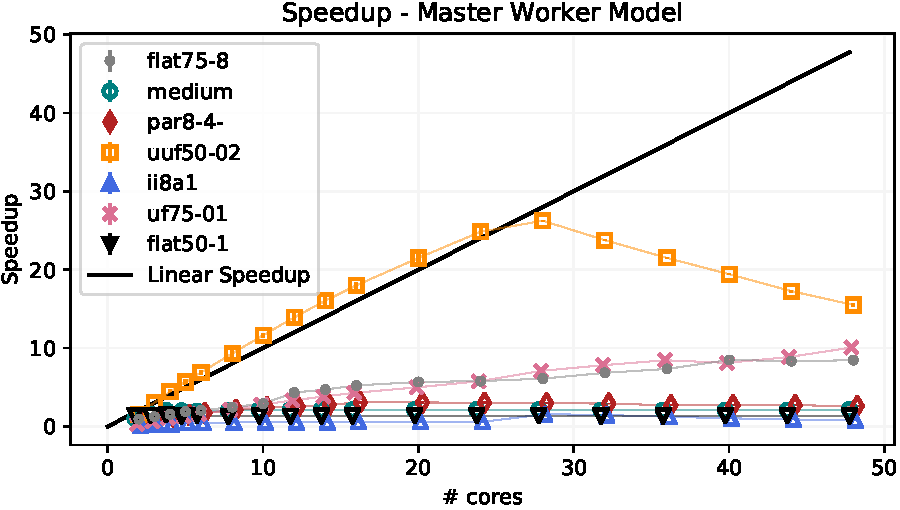
\includegraphics[width=\columnwidth]{figures/scaling_parallel_non_subset_dpll_scaling_tar.pdf}
    \caption{Average speedup of master worker parallel DPLL implementation compared to sequential DPLL.
    Second subset.}
    \label{fig:dpll_parallel_speedup_non}
\end{figure}

\begin{figure}[p]
    \centering
    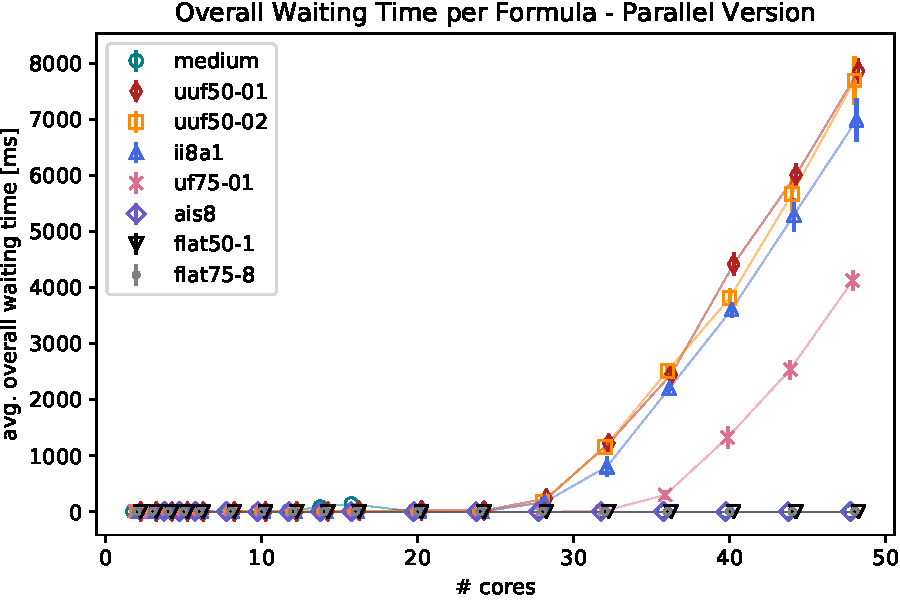
\includegraphics[width=\columnwidth]{figures/waiting_parallel_non_subset_dpll_scaling_tar.pdf}
    \caption{Average overall waiting time of workers per cnf in the master worker model.
    All waiting times per worker are summed up.
    Second subset.}
    \label{fig:dpll_parallel_waiting_non}
\end{figure}

\begin{figure}[p]
    \centering
    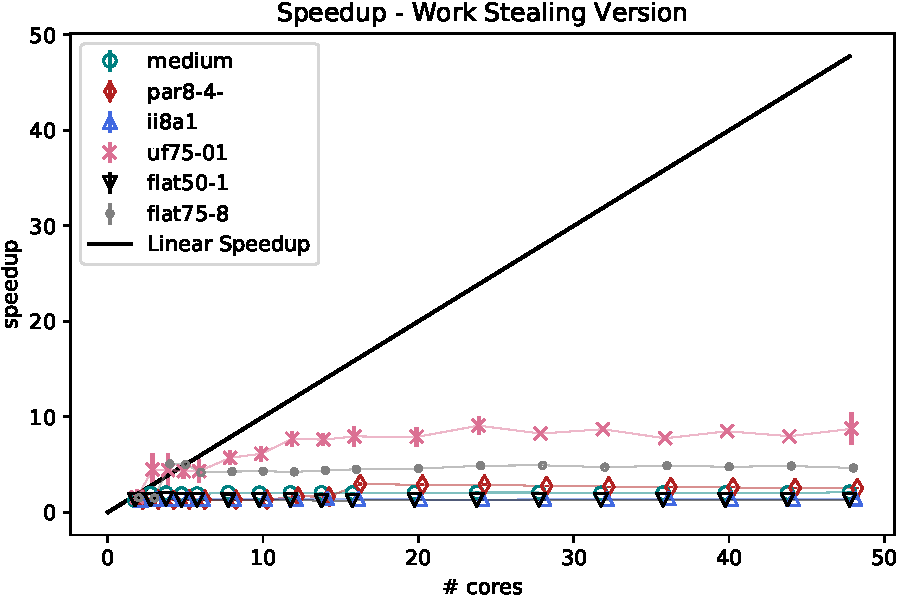
\includegraphics[width=\columnwidth]{figures/scaling_stealing_non_subset_dpll_scaling_tar.pdf}
    \caption{Average speedup of working stealing parallel DPLL implementation compared to sequential DPLL.
    Second subset.}
    \label{fig:dpll_stealing_speedup_non}
\end{figure}

\begin{figure}[p]
    \centering
    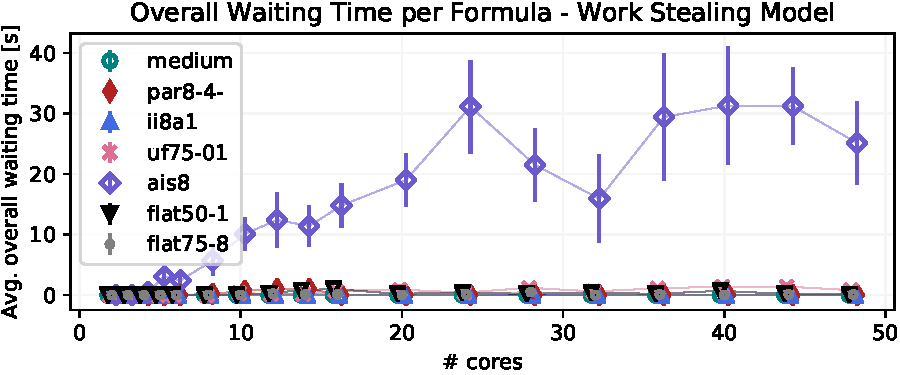
\includegraphics[width=\columnwidth]{figures/waiting_stealing_non_subset_dpll_scaling_tar.pdf}
    \caption{Average overall waiting time of workers per cnf in the work stealing model.
    All waiting times per worker are summed up.
    Second subset.}
    \label{fig:dpll_stealing_waiting_non}
\end{figure}

\begin{figure}[p]
    \centering
    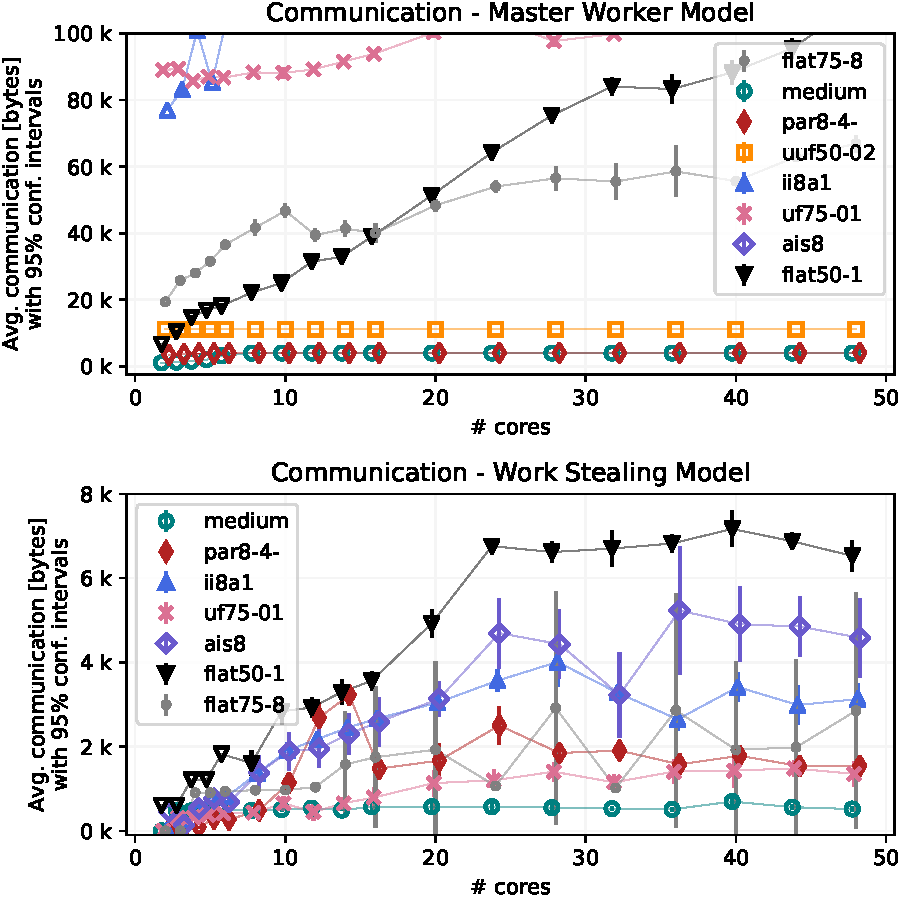
\includegraphics[width=\columnwidth]{figures/comm_non_subset_dpll_scaling_tar.pdf}
    \caption{Overall amount of transferred bytes for both the master worker model and the stealing model.
    Second subset.}
    \label{fig:comm_reduce_non}
\end{figure}

\begin{figure}[h]
    \centering
    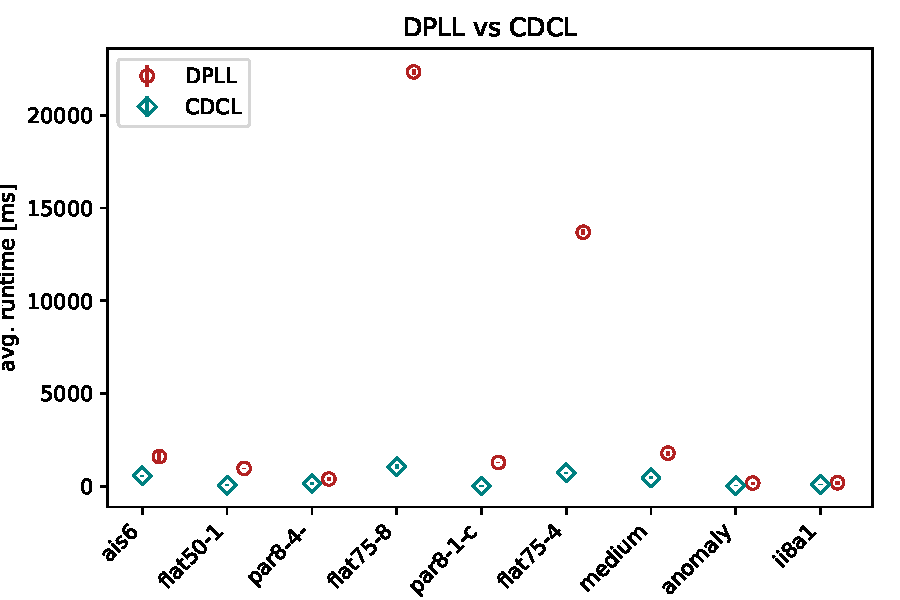
\includegraphics[width=\columnwidth]{figures/dpll_vs_cdcl.pdf}
    \caption{DPLL vs CDCL sequential runtime. Average runtime with 95\% confidence intervals.}
    \label{fig:dpll_vs_cdcl}
\end{figure}

\begin{table}[p]
    \centering
    \begin{tabularx}{\columnwidth}{|p{1.3cm}|X|p{2.2cm}|}
        \hline
        Formula & Best Solver Configuration & Runtime [ms]\\
        \hline
        \hline
        anomaly & CDCL sequential & 16.2 $\pm$ 4.18 \\
        \hline
        medium & CDCL sequential & 414.8 $\pm$ 32.94 \\
        \hline
        ais6 & DPLL master worker, 14 cores & 343.3 $\pm$ 3.58 \\
        \hline
        ais8 & DPLL master worker, 48 cores & 3015.3 $\pm$ 58.85 \\
        \hline
        flat50-1 & CDCL sequential & 36.4 $\pm$ 9.07 \\
        \hline
        flat75-4 & CDCL sequential & 702.8 $\pm$ 38.18 \\
        \hline
        flat75-8 & CDCL sequential & 1054.2 $\pm$ 50.72 \\
        \hline
        ii8a1 & DPLL master worker, 6 cores & 72.2 $\pm$ 0.79 \\
        \hline
        par8-1-c & CDCL sequential & 15.2 $\pm$ 2.28 \\
        \hline
        par8-4- & DPLL master salve, 2 cores & 132.2 $\pm$ 2.22 \\
        \hline
        uf50-01 & CDCL sequential & 31.5 $\pm$ 9.21 \\
        \hline
        uf75-01 & DPLL master worker, 32 nodes & 297.4 $\pm$ 7.99 \\
        \hline
        uuf50-01 & DPLL master worker 24 nodes & 187.5 $\pm$ 5.59 \\
        \hline
        uuf50-02 & DPLL master worker 24 nodes & 148.9 $\pm$ 2.85 \\
        \hline
    \end{tabularx}
    \caption{Benchmark formulas with best performing configuration.}
    \label{tab:cnfs_parallel}
\end{table}

\end{document}
